\documentclass[10pt]{beamer}
\usetheme[
%%% option passed to the outer theme
%    progressstyle=fixedCircCnt,   % fixedCircCnt, movingCircCnt (moving is deault)
  ]{Feather}
  
% If you want to change the colors of the various elements in the theme, edit and uncomment the following lines

% Change the bar colors:
%\setbeamercolor{Feather}{fg=red!20,bg=red}

% Change the color of the structural elements:
%\setbeamercolor{structure}{fg=red}

% Change the frame title text color:
%\setbeamercolor{frametitle}{fg=blue}

% Change the normal text color background:
%\setbeamercolor{normal text}{fg=black,bg=gray!10}

%-------------------------------------------------------
% INCLUDE PACKAGES
%-------------------------------------------------------

\usepackage[utf8]{inputenc}
\usepackage[english]{babel}
\usepackage[T1]{fontenc}
\usepackage{helvet}

%-------------------------------------------------------
% DEFFINING AND REDEFINING COMMANDS
%-------------------------------------------------------

% colored hyperlinks
\newcommand{\chref}[2]{
  \href{#1}{{\usebeamercolor[bg]{Feather}#2}}
}

%-------------------------------------------------------
% INFORMATION IN THE TITLE PAGE
%-------------------------------------------------------

\title[] % [] is optional - is placed on the bottom of the sidebar on every slide
{ % is placed on the title page
      \textbf{\bf MATRIX PROJECT}
}

\subtitle[MATRIX PROJECT]
{
      \textbf{MATRIX PROJECT}
}

\author[C SHRUTI \& SHRESHTA.T]
{      C SHRUTI \& SHRESHTA.T \\
      {}
}

\institute[]
{
     IIT HYDERABAD
  
  %there must be an empty line above this line - otherwise some unwanted space is added between the university and the country (I do not know why;( )
}

\date{\today}

%-------------------------------------------------------
% THE BODY OF THE PRESENTATION
%-------------------------------------------------------

\begin{document}

%-------------------------------------------------------
% THE TITLEPAGE
%-------------------------------------------------------

{\1% % this is the name of the PDF file for the background



\begin{frame}{MATRIX PROJECT}{}


{\bf INTRODUCTION TO AI AND ML}
\newline

EE1390
\newline

\bullet C.SHRUTI 
\newline

\bullet SHRESHTA.T \end{frame}

%-------------------------------------------------------
\section{Question}
%-------------------------------------------------------
\subsection{JEE MAIN 2007}
\begin{frame}{Question}{JEE MAIN 2007}
%-------------------------------------------------------

   The equation of a tangent to the parabola 
   \begin{equation}
       y^2=8x
   \end{equation}  
   is 
   \begin{equation}
    y=x+2   
   \end{equation}Find the point on this line from which the other tangent to the parabola is perpendicular to the given tangent. 
    
  
\end{frame}
\begin{frame}{Question}{JEE MAIN 2007}
The equation of a tangent to the parabola
\begin{equation}
{\bf X}^T
\begin{bmatrix}
0 & 0\\
0 & 1
\end{bmatrix}    
{\bf X}+\begin{bmatrix}
-8&&0\\
\end{bmatrix}
{\bf X}=0
\end{equation}
is 
\begin{equation}
\begin{bmatrix}
1 & -1
\end{bmatrix}
{\bf X}=-2
\end{equation}
Find the point on this line from which the other tangent to the parabola is perpendicular to the given tangent.
\end{frame}

%-------------------------------------------------------
\begin{frame}{FIGURE}
\begin{figure}
    
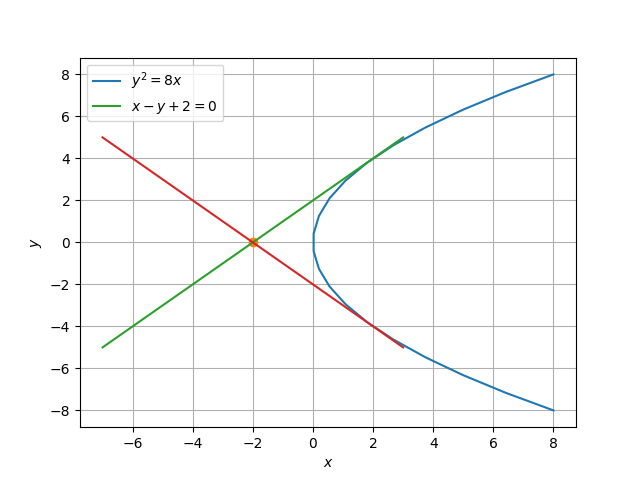
\includegraphics[scale=0.6] {figure3.png}
\end{figure}    
\end{frame}
\begin{frame}{SOLUTION}{METHOD-1}
    Given equation of the line in matrix form :\begin{bmatrix}
    1&-1\\
    \end{bmatrix}{\bf X}= -2
    
Tangent to a standard parabola is of the form \begin{bmatrix}
m&-1
    \end{bmatrix}{\bf X}= (-a/m)
    Normal vector of the line specified = {\bf A} and given that the other tangent is perpendicular to this line.
    Let the normal vector of the other tangent be {\bf B}.
    Now {\bf A} and {\bf B} are orthogonal  i.e.. {\bf A}^T {\bf B} =0 
    
    \begin{bmatrix}
    1 & -1 \\
    \end{bmatrix}
    \begin{equation}
    \begin{bmatrix}
    m \\
    -1
    \end{bmatrix}
    =0
    \end{equation}
    \begin{equation}
    m=-1    
    \end{equation}
    
\end{frame}


%-------------------------------------------------------

\begin{frame}{SOLUTION}{METHOD-1}
%-------------------------------------------------------
  
 Equation of perpendicular tangent:
 \begin{bmatrix}
 -1 & -1\\
 \end{bmatrix}
{\bf X} = 2
\newline
 \begin{bmatrix}
 1 & -1\\
 \end{bmatrix}
 {\bf X} = -2
 \newline
 
Point of intersection of two tangent:
\[
\begin{bmatrix}
-1 & 1\\
-1 & -1
\end{bmatrix}
{\bf X} =
\begin{bmatrix}
2\\
-2
\end{bmatrix}
\]

\centering
\begin{bmatrix}
x\\
y
\end{bmatrix}
= 1/2
\begin{bmatrix}
-1 & -1\\
1 & -1
\end{bmatrix}
\begin{bmatrix}
2\\
-2
\end{bmatrix}
\newline

x = -2, y = 0
\end{frame}

    
\begin{frame}{FIGURE FOR THE SOLUTION}
\begin{figure}
    
    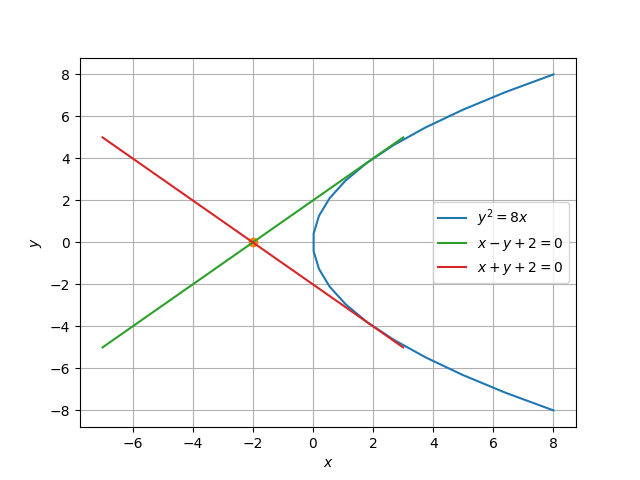
\includegraphics[scale=0.6]{figure1.png}
    
\end{figure}    
\end{frame}  

%-------------------------------------------------------

\begin{frame}{SOLUTION}{METHOD-2}
%-------------------------------------------------------
From the properties of parabola ,we know that the locus of point of intersection of perpendicular tangents to the parabola is given by the directrix of the parabola.
The equation to the directrix of the standard parabola is [1 0]{\bf X} = -a
 
\end{frame}

%-------------------------------------------------------
\section{SOLUTION}
\subsection{METHOD-2}
\begin{frame}{SOLUTION}{METHOD-2}
%-------------------------------------------------------
 For the given parabola 
 y^2 = 8x , a = 2 

 \newline
 
 Hence the  equation of the directrix becomes [1  0]{\bf X} = -2.
 Let the required  point of intersection be [h k].
 h = -2 as it lies on the directrix.
 
\end{frame}

\begin{frame}{SOLUTION}{METHOD-2}
Now, since \begin{bmatrix}
-2\\
k
\end{bmatrix} lies on the line [1  -1]{\bf X} = -2, substituting {\bf X}= \begin{bmatrix}
-2\\
k
\end{bmatrix} gives us the equation,
-2 + k = -2 i.e.. k = 0.
Hence the point is (-2,0).
  
\end{frame}
\section{FIGURE}
\begin{frame}{FIGURE FOR THE SOLUTION}
    \begin{figure}
    
    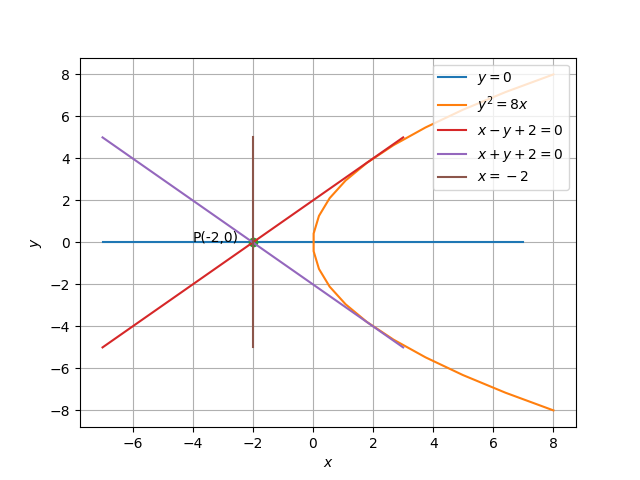
\includegraphics[scale=0.6]{figure2.png}
    
\end{figure} 
\end{frame}


\end{document}
